%\documentclass[a4paper]{article}
\documentclass{article}
\usepackage[letterpaper,top=2cm,bottom=2cm,left=3cm,right=3cm,marginparwidth=1.75cm]{geometry}

% === Useful packages ===
\usepackage[german]{babel}
\usepackage[letterpaper,top=2cm,bottom=2cm,left=3cm,right=3cm,marginparwidth=1.75cm]{geometry}

\usepackage{amsmath}
\usepackage{graphicx}
% \usepackage[colorlinks=true, allcolors=blue]{hyperref}

% --- manage multicols ---
\usepackage{multicol}
% \setlength{\columnsep}{Xpt}
\setlength{\columnseprule}{1pt}

\usepackage{paracol} % cause multicol does not work properly over several pages I have to use paracol
% \setlength{\columnsep}{Xpt}
% \setlength{\columnseprule}{1pt}

\title{Signal und System Theorie}
\author{Prof. Dr.-Ing. Frank Giesecke}
\date{}

\begin{document}
\maketitle

\section*{28.10.2024}

\subsection*{Wiederholung}

\begin{enumerate}
\item Leistungssignale \\
Gleichanteil/ linearer Mittelwert/ Moment 1. Ordnung \\
$\Bar{x} = (coming_soon)$
\[
    f(x) = \lim_{T\to\infty} \int_{-T}^{T} x^2 \,dt 
\]

\item Signalgleichleistung \\
(Leistung, die den Gleichanteil verursacht) \\
$P_{x=} = \Bar{x}^2 = m_1^2$

\item mittlere Signalleistung/ quadratische Mittelwert/ Gesamt-Signalleistung / Moment 2. Ordnung \\
$P = \Bar{x^2} = m_2 = (coming_soon)$

\item Effektivwert (Wurzel aus der mittleren Signalleistung) \\
$x_{eff}=\sqrt{P}=\sqrt{x^2}$

\item Signalwechselleistung/ Varianz/ Zentral-Moment 2. Ordnung \\
$P_{x~}=\sigma^2 = \mu_2 = P_x - P_{x=} = \Bar{x^2} - \Bar{x}^2$

\item Standartabweichung \\
$\sigma = \sqrt{P_{x~}} = \sqrt{\mu_2}$
\end{enumerate}

\subsection*{Alternative Berechnung der Signalwechselleistung/ Varianz/ Zentral-Moment 2. Ordnung}
$P_{x~} = (coming_soon)$ \\
$P_{x~} = P_x - P_x$

\subsection*{Direkte Berechnung der Varianz/ Signalwechselspannung aus einem Datensatz (digital)}

\begin{center}
    Fallunterscheidung
\end{center}
\begin{multicols}{2}
    linerer Mittelwert/ Gleichanteil ist bekannt oder kann exakt bestimmt werden. \\
    $\Bar{x} ist bekannt$ \\
    $\sigma^2 = P_{x~} = \mu_2 = (coming_soon)$
    
    \columnbreak
    linearer Mittelwert wird aus den N Werten bestimmt. \\
    $\Bar{x} ist un-bekannt$ \\
    $\Bar{x_N} = (coming_soon)$ \\
    $\sigma^2 = P_x = (coming_soon)$
    
\end{multicols}
\begin{center}
    N = Anzahl der Werte
\end{center}

\subsection*{Es folgt:}
Angenäherter Einheitssprung, Einheitssprung-Funktion, Einheitsimpuls-Funktion, Deltaimpuls/ Dirac-Impuls, Einheitsanstiegs-Funktion

\subsection*{Angenäherter Einheitssprung ($\delta$ delta)}
\begin{multicols}{3}
    (grafic is coming soon)

    \columnbreak

    \begin{center}
    $\overrightarrow{Differentation}$ \\
    $(\frac{d}{dt})$ \\
    \vspace{1em}
    $\overleftarrow{Integration}$ \\
    $\hookrightarrow$ Intigrationsgrenzen \\
    $-\infty bis aktueller Zeitpunkt (t)$ \\
    $\sigma = (coming_soon)$
    \end{center}

    \columnbreak
    (grafic is coming soon)
\end{multicols}

\section*{\centering **.**.2024 Vorlesung noch nicht nachgetragen}


\newpage
\section*{\centering 11.11.2024}
\subsection*{Ergänzung: Kreuzrelation}

\[
    E_{x1x2}(\tau)=\int_{-\infty}^{\infty}x(t)*x_2(t+\tau)*dt
\]
mindestens eines der Verläufe muss ein Energiesignal sein. \\
Wenn beide Verläufe $x_1$ und $x_2$ Leistungssignale sind, dann:
\[
    Allg. Variante: P_{x1x2}(\tau)=\lim_{T\to\infty}x_1(t)x_2*x_2(t+\tau)*dt
\]

    bei Vorliegen einer Periodizität von $x_1$ und $x_2$
\[
    P_{x1x2}(\tau)=\frac{1}{T}\int_{0}^{T}x(t)*x_2(t+\tau)*dt
\]
entweder T als gleiche Periode bei den Verläufen oder T als gemeinsames Vielfaches der beiden Periodenduaer von $x_1$ und $x_2$

\subsection*{\centering Das System}
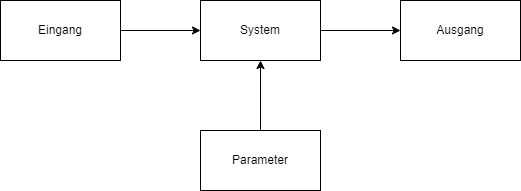
\includegraphics[scale=0.8]{img/2024_11_11.png}

\subsubsection*{Im Zeitbereich:}
z.B. Spannung $u_e(t) \to u_a(t)$ \\
oder digital/zeitdiskret

\subsubsection*{System im Laplace Bereich}
$s=\sigma+j\omega$ \\
(system im laplace-bereich bild fehlt wurde aber schon erstellt)

\subsubsection*{System in Frequenzbereich}

\subsubsection*{System-Eigenschaften}
4 Grundeigenschaften:
\begin{itemize}
    \item Linearität
    \begin{itemize}
        \item linear
        \item licht linear
    \end{itemize}
    
    \item Zeitinvarianz
    \begin{itemize}
        \item Zeit-konstant
        \item Zeit-veränderlich
    \end{itemize}
    
    \item Kausalität
    \begin{itemize}
        \item kausal
        \begin{itemize}
            \item statisch (speicherlos)
            \item dynamisch (mit Speicherelementen)
        \end{itemize}
        \item a-kausal (nicht kausal)
    \end{itemize}
    
    \item Stabilität
    \begin{itemize}
        \item Stabil
        \item Grenz-Stabil
        \item In-Stabil
    \end{itemize}
\end{itemize}


\newpage
\section*{13.11.2024 (fehlt)}
war krank und muss noch nachtragen


\newpage
\section*{\centering 18.11.2024 (fehlt)}
die Aufzeichnung dieser Stunde habe ich auf dem Papier gemacht und muss noch nachgetragen werden.

\newpage
\section*{\centering 20.11.2024}
\subsection*{Stabilitätsbestimmung über die Übertragungsfunktion}
\begin{itemize}
	\item analoge/zeitkontinuierliche Systeme $G(s)$ Übertragungsfunktion \\
	s: Laplace Variable \\
	$s=\delta+j\omega$
	\item digitale/zeitdiskrete Systeme $G(z)$ Übertragungsfunktion \\
	z: z-Variable \\
	$z=Re(z) + j * Im(z) = |z| * e^{j*\phi_z} $
\end{itemize}
Nullsetzen des ZählerTerms $(G(s) bzw. G(z))$ liefert die Nullstellen \\
Nullsetzen des Nenner-Terms $(G(s) bzw. G(z))$ liefert die Polstelle \\
Wenn eine Nullstelle nicht genau auf eine Polstelle fällt haben die Nullstellen keinen Einfluss auf die Stabilität. \\
Wenn eine Nullstelle genau auf eine Polstelle fällt, wird die entsprechende Polstelle ausgelöscht.
\begin{center}
Bsp.:
\[
G(s) = \frac{ (s-s_{01}) * (s-s_{0n}) }{ (s-s_{p1}) * (s-s_{pn}) }*K
\]
\end{center}

\subsubsection*{Betrachtung der verbleibenden (nicht durch Nullstellen ausgelöschten) Polstellen zur Stabilitätsbestimmung}
Betrachtung der Lage der Polstellen in den Ebenen
\begin{paracol}{2}
$G(s) \rightarrow$  s-Ebene \\
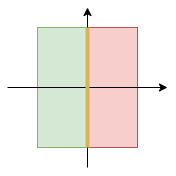
\includegraphics[scale=0.8]{img/2024_11_20_s-Ebene.png}
\begin{itemize}
	\item Polstellen link von der $j\omega$-Achse \\
	$\rightarrow$ System ist Stabil
	\item mindestens eine Polstelle rechts der $j\omega$-Achse oder mindestens eine mehrfache Polstelle auf der $j\omega$-Achse \\
	$\rightarrow$ System ist stabil
	\item keine Posstelle rechts der $j\omega$-Achse und nur einfache Polstellen (beliebiger Anzahl an unterschiedlichen Stellen) \\
	$\rightarrow$ System ist grenzstabil
\end{itemize}
\paragraph{Bsp. Integrator}
\[
E \rightarrow G_I(s)=\frac{1}{s} = s^{-1} \rightarrow A
\]
2 Intigratoren in Kette:
\[
E \rightarrow s^{-1} \rightarrow s^{-1} \rightarrow A
\]
$\rightarrow$ 2 grenzstabile Systeme werden zusammen 1 instabiles System

\switchcolumn

$G(z) \rightarrow$ z-Ebene \\
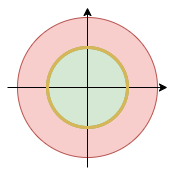
\includegraphics[scale=0.8]{img/2024_11_20_z-Ebene.png}
\begin{itemize}
	\item alle Polstellen innerhalb des Einheitskreises (nicht auf dem Einheitskreis) \\
	$\rightarrow$ System ist stabil
	\item mindestens eine Polstelle außerhalb des Einheitskreises oder mindestens eine mehrfache Polstelle auf dem Einheitskreis \\
	$\rightarrow$ System ist stabil
	\item keine Polstelle außerhalb des Einheitskreises und nur einfache Polstellen (beliebiger Anzahl an unterschiedlichen Stellen) auf dem Einheitskreis \\
	$\rightarrow$ System ist grenzstabil
\end{itemize}
\paragraph{Bsp. Integrator}
\[
E \rightarrow s^{-1} \rightarrow s^{-1} \rightarrow A
\]
\[
G_{ges} = G_1(s) * G_2(s) = s^{-2}
\]
doppelte Polstelle bei 0 \\
$\rightarrow$ 2 stabile Systeme werden zusammen 1 instabiles System
\end{paracol}


\newpage
\section*{\centering 25.11.2024}
\subsection*{Anforderung an die Systemeigenschaften zur Anwendbarkeit von Werkzeugen der Systemtheorie}
Beschreibung eines Systems durch:
\begin{itemize}
	\item Impulsantwort: $g(t), g(k)$; Sprungantwort: $h(t), h(k)$; Anstiegsanwort: $a(t), a(k)$ \\
	System muss linear und zeitinvariant sein. \\
	(Kausalität und Stabilität sind beliebig)
	\begin{center}
		$h(t) = \int_{0}^{t}g(t)*d\tau$ \\
		$g(t) = \frac{dh(t)}{dt}$
	\end{center}
	
	\item Übertragungsfunktion: $G<(s)$ (Laplace), $G(z)$ (z-Transformation) \\
	System muss linear, zeitinvariant und kausal sein. \\
	(Stabilität spielt keine Rolle)

	\item Komplexer Frequenzgang $G(j\omega)$, $G(\omega)$, G(jf), G(f) bzw. G(m) \\
	System muss linear, zeitinvariant und stabil oder grenzstabil sein. \\
	(Kausalietät spielt keine Rolle)
	\begin{center}
		Fourier-Transformation: $g(t) \rightarrow G(j\omega)$ \\
		Diskrete-Fourier-Transformation: $g(t) \rightarrow G(m)$
	\end{center}
\end{itemize}

\paragraph{Querverbindung:}
$G(s) \rightarrow G(j\omega)$, $G(\omega)$,  G(jf) oder G(f) \\
$s=\delta + j\omega \rightarrow \delta = 0$\\
Nur bei einem stabilen oder Grenzstabilen System erlaubt.

\subsection*{Ausgang eines linearen und zeitinvarianten Systems zur System-Charakterisierung}
\paragraph{Deltaimpuls} ist am besten geeignet weil: 
\begin{itemize}
	\item besitzt alle Frequenzanteile
	\item alle Frequenzanteile haben die selbe Intensität
\end{itemize}
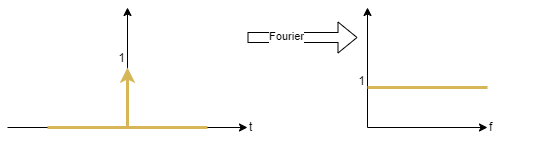
\includegraphics[scale=0.8]{img/2024_11_25_fourier_deltaimpuls.png}

\paragraph{Einheitssprung:} \mbox{} \\
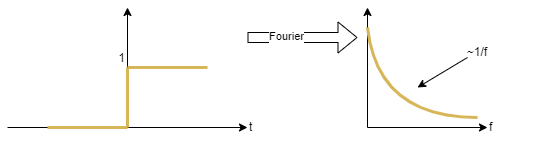
\includegraphics[scale=0.8]{img/2024_11_25_fourier_einheitssprung.png}

\paragraph{Einheitsanstieg:} \mbox{} \\
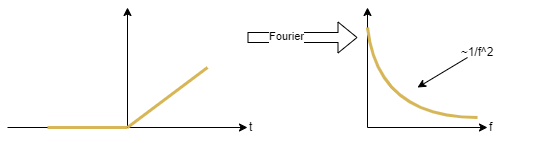
\includegraphics[scale=0.8]{img/2024_11_25_fourier_einheitsanstieg.png}

\subsection*{Ermittlung des Ausgangssignals aus einem Eingangssignal bei bekannter Impulsantwort g(t) bzw. g(k)}
Eingangssignal x(t) $\rightarrow$ System g(t) $\rightarrow$ Ausgangssignal y(t)

\paragraph{Faltungsoperation (*):}
\begin{center}
$ y(t) = x(t) * g(t)$ \\
(Faltung wird durch Transformation zur komplexen Multiplikation) \\
\mbox{} \\
$y(t) = x(t) * g(t) = \int_{-\infty}^{\infty} x(t) * g(-\tau + t) d\tau$ \\
(äquivalent mit Summe für zeitdiskrete Systeme)
\end{center}

\paragraph{Kreuzkorrelation (schon mal gemacht)}
\begin{center}
$E_{x_1x_2}(\tau) = \int_{-\infty}^{\infty} x_1(t) * x_2(t + \tau) * dt$ \\
(Im prinzip das selbe wie die Faltungsoperation nur mit einer anderen Intention)
\end{center}


\end{document}














